\section{System Architecture} \label{sec:system-architecture}

In this section we describe the underlying inverted index architecture, query
operators, query processing and offline replay framework used to build job
search and recommendations at LinkedIn. Both search and recommendations are
powered by an inverted index. The underlying engine is custom build called
Galene~\cite{sriram2014}. Galene still uses the indexing format of the open
source search engine Lucene~\cite{mccandless2010lucene}. The Lucene primitives
are used to build the index, construct queries and retrieve matching documents.
All other components are custom built. The major components/features of our
architecture are as follows:

\subsection{Indexing}
Indexing on Hadoop~\cite{white2012hadoop} takes the form of multiple map-reduce operations that progressively refine the data into the data models 
and search index that ultimately serve live queries (Figure~\ref{fig:offline-indexing}).  
HDFS contains raw data containing all the information we need to build the index.  
We first run map reduce jobs with standardization algorithms that enrich the raw data resulting in the derived data.  
The raw data goes through standardization where it gets converted to structured
entities. For example, a job posting may have the following free form
description {\it ``Looking for Software Engineers with 5+ years' experience in
Java''}. Standardization would extract the fact that the job requires a skill
called {\it \bf ``java''} and store that directly as a field in the index. 

\subsection{Early Termination}
Galene provides the ability to assign a static rank to each entity.  This is a measure of the importance of that 
entity independent of any search query, and is determined offline during the index building process.  
Using the static rank, we order the entities in the index by importance, placing the most important entities for a term first.  
The retrieval process can then be terminated as soon as we obtain an adequate number of entities that match the query, 
and not have to consider every entity that matches the query.  This strategy is called 
early termination~\cite{anh2001vector,yan2010efficient,zhang2010revisiting}.
Early termination works if the static rank of an entity is somewhat correlated to its final score for any query.  
The main benefit of early termination is performance, scoring is usually an expensive operation and the fewer the entities scored the better.  
Looked at in another way, early termination allows us to use more sophisticated scorers. Consider a broad query term like ``marketing''. 
Assume that we are looking for the term in the job description, a traditional
query would look like this: 

\lucenequery{+DESCRIPTION: marketing }

The above query implies the following - {\it retrieve those documents that MUST
have the term ``marketing'' in the field DESCRIPTION}. Note that this would
retrieve prohibitively high number of documents. Let's say we only rank
$numToScore$.
documents. We could rewrite the query using early termination as:

\lucenequery{+DESCRIPTION: marketing[numToScore]}

The above query implies - {\it retrieve those documents that MUST
have the term ``marketing'' in the field DESCRIPTION, but stop after retrieving
the first numToScore documents}

For the rest of the paper we shall refer to early termination as $numToScore$. 

\subsection{WAND and FLEX operators} \label{sec:wand}

Our retrieval engine gives us the capability to do two powerful operators -
WAND and FLEX.

Consider the simple example where the index has three fields - TITLE,
DESCRIPTION and SKILL. Assume that the query is ``marketing''. One way
to rewrite this query is:

\lucenequery{+(?TITLE:marketing ?SKILL:marketing \\
\quad ?DESCRIPTION:marketing)}

The above query would imply fetching documents which match the term ``marketing'' in {\it
any} of the fields and let the ranking function identify the top documents. This could be
prohibitively expensive and it may retrieve irrelevant documents. Suppose we
have a way to construct the following query {\it retrieve all documents which
match at least one of the two fields in (TITLE, SKILL, DESCRIPTION)}, it would
significantly reduce both the number of irrelevant documents as well as
latency. It will reduce the work load on the top level ranking function.

WAND operators provide such flexibility~\cite{broder2003efficient}. More
formally assume that $ X = (x_1, x_2 \ldots x_n)$ represents $n$ query operators
associated with weights $ W = (w_1, w_2, \ldots w_n)$. WAND($X$, $W$)
is true iff:
\begin{equation}
    \sum_{1 \leq i \leq k} t_i w_i >= \theta
\label{eqn:wand}
\end{equation}
$t_i$'s are Boolean variables that are set to 1 if clause $x_i$ is satisfied
and 0 otherwise. 

For the query ``marketing'', consider a WAND query of the following form:

$X$ = \lucenequery{(?TITLE:marketing, ?SKILL:marketing, \\
?DESCRIPTION:marketing)}

$W$ = (1, 1, 1)

$\theta$ = 2


In the WAND formulation shown above, {\bf at least
two clauses out of the fields must match} for the document to be retrieved. This
significantly reduces the number of irrelevant documents retrieved.
We will later describe how we train the weights of the WAND clauses using
decision trees. 

To motivate the need for FLEX operator, consider the example where the query is
``oracle''. We understand that the term ``oracle'' represents a company with
very high probability. So, the query could be written as:

\lucenequery{+COMPANY:oracle}[1000]

The above query retrieves at most 1000 documents where the company field MUST
match the term ``oracle''. Rewriting the query to retrieve only documents which
match the company field assumes that we got the intent of the user right 100\%
of the time. In this case, sometimes the user may have meant ``oracle db'' or
something else. Let's say that the user intent while typing a query like
``oracle'' is to find jobs at the company Oracle 99\% of the time and mean
something else 1\% of the time. FLEX operator provides the flexibility to handle
such cases. 

More formally given $k$ conjunctive query clauses $X = (x_1, x_2 \ldots x_k)$ and
$k$ weights $W = (W_1, W_2, \ldots W_k)$, let $d_i$ represent the number of
documents where the clause $X_i$ is satisfied, then retrieval will continue
until the following conditions are met or all documents are considered:

\begin{equation} \label{eqn:flex}
    d_i \geq w_i \quad \forall 1 \leq i \leq k
\end{equation}

In the example for ``oracle'', let us assume that the query represents a
company {\it Oracle} with 99\% probability and skill with 1\% probability.
Then we could set:

$X = \lucenequery{+(?COMPANY:oracle, ?SKILL:oracle)}$

$W = (990, 10)$ 

This
would ensure at least 10 documents retrieved where the term ``oracle'' is a
match in the skills field.

\subsection{Replay Framework} \label{sec:replay-framework}

\begin{figure*}
\centering
%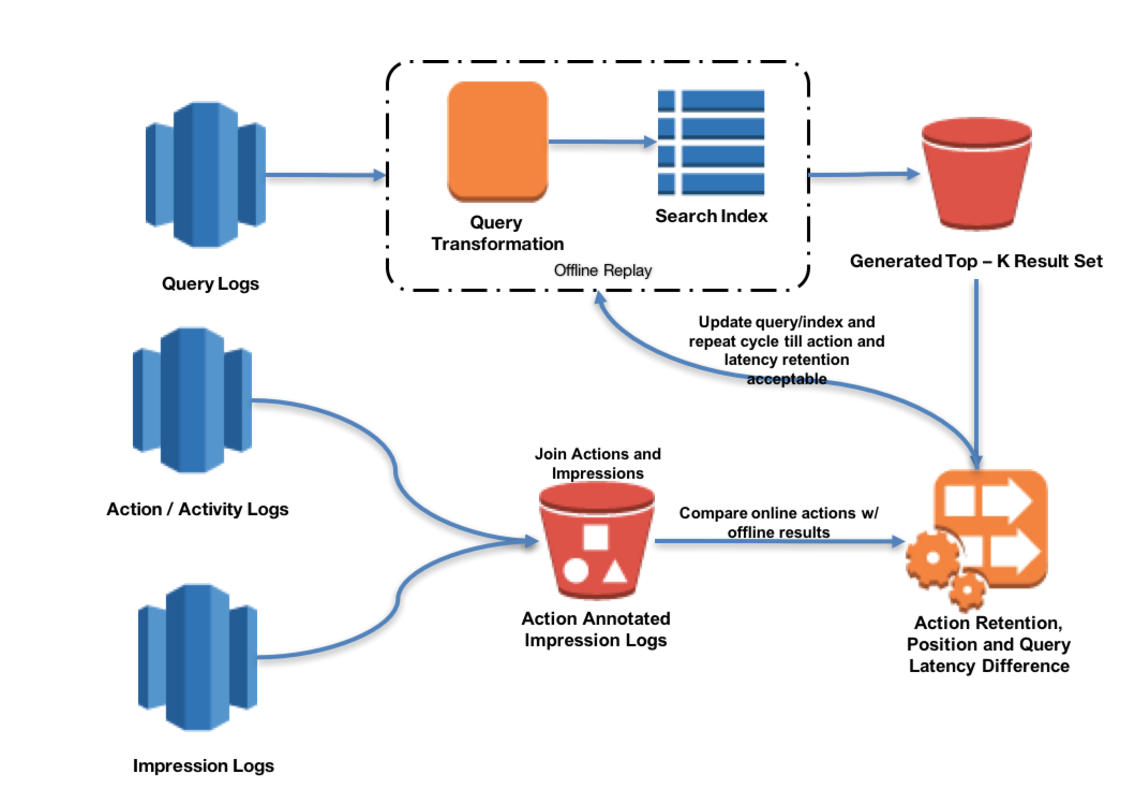
\includegraphics[width=\textwidth,scale=0.50]{replay-architecture.png}
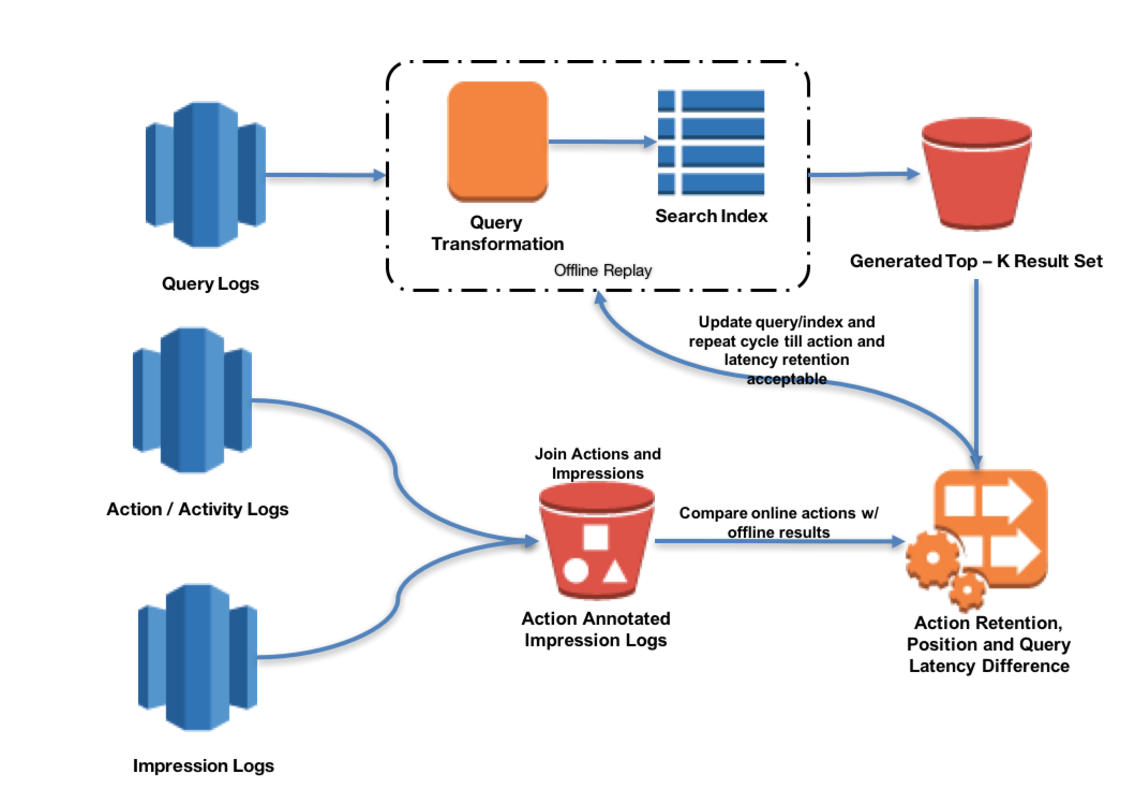
\includegraphics[scale=0.90]{replay-architecture.png}
\caption{Replay Framework}
\label{fig:replay-architecture}
\end{figure*}

At the core of the query construction process is an offline replay framework
shown in Figure~[\ref{fig:replay-architecture}]. This helps us in validating how we 
are doing compared to the baseline candidate selection model as well as to only 
take the best and validated queries to production.
We document the individual components that are part of the replay cycle and show 
examples from job recommendations vertical.

\subsubsection{Query, Impression and Activity Tracking}

For the replay of the queries we require support to track the query that 
was done online along with the results that were retrieved, ranked and 
shown to the members and guests. The tracking requires the exact retrieval 
query to be tracked. 
The exact query allows us to make modifications to query construction 
and use the same in the replay framework. This removes the need 
for regenerating the query with all member and job features and be sure 
what query was used to generate the tracked results. 

The tracked results are annotated with the specific actions that are needed 
for evaluation in the replay framework. As an example, in case of job 
recommendations we track job views and applications, and dismiss actions 
for each of the tracked job recommendations. 

\subsubsection{Offline Replay}
The offline replay can be broken down into the following steps: 
\begin{itemize}
\item Online data aggregation
\item Query log preparation
\item Query log replay
\item Analysis of replay results 
\end{itemize}

It utilizes the online query logs and runs a transformation to allow operations such as
query construction, replaying ranking with particular models etc.

The original queries are parsed through the query transformer and 
new candidate selection model is added into the query config. 
As the next step, we take both the modified queries as well as the original 
queries and replay them on hadoop using offline retrieval infrastructure (known
as {\bf offline Galene})

The results collected through the replay are then passed to a result 
comparator which goes through both the baseline and new rank-list and 
computes the action retention metrics. As an example, in the case of job 
recommendations we compute. 
\begin{itemize}
\item Job View/Application/Dismiss Retention
\item Number of hits scored
\end{itemize}

As an additional step, we also compute the difference between the baseline and 
modified queries to see what jobs that had actions were missed. 
This allows us to revisit the candidate selection model to debug why we 
missed retrieving the jobs. 

The workflow is implemented in a generic manner 
in Hadoop and can be utilized for tasks outside of query construction such 
as training data generation, model validation and rank-list metrics computation. 
